\documentclass[journal,12pt,twocolumn]{IEEEtran}

\usepackage{setspace}
\usepackage{gensymb}

\singlespacing


\usepackage[cmex10]{amsmath}

\usepackage{amsthm}

\usepackage{mathrsfs}
\usepackage{txfonts}
\usepackage{stfloats}
\usepackage{bm}
\usepackage{cite}
\usepackage{cases}
\usepackage{subfig}


\usepackage{longtable}
\usepackage{multirow}

\usepackage{enumitem}
\usepackage{mathtools}
\usepackage{steinmetz}
\usepackage{tikz}
\usepackage{circuitikz}
\usepackage{verbatim}
\usepackage{tfrupee}
\usepackage[breaklinks=true]{hyperref}
\raggedbottom

\usepackage{tkz-euclide}

\usetikzlibrary{calc,math}
\usepackage{listings}
    \usepackage{color}                                            %%
    \usepackage{array}                                            %%
    \usepackage{longtable}                                        %%
    \usepackage{calc}                                             %%
    \usepackage{multirow}                                         %%
    \usepackage{hhline}                                           %%
    \usepackage{ifthen}                                           %%
    \usepackage{lscape}     
\usepackage{multicol}
\usepackage{chngcntr}
\graphicspath{ {./images/} }

\DeclareMathOperator*{\Res}{Res}

\renewcommand\thesection{\arabic{section}}
\renewcommand\thesubsection{\thesection.\arabic{subsection}}
\renewcommand\thesubsubsection{\thesubsection.\arabic{subsubsection}}

\renewcommand\thesectiondis{\arabic{section}}
\renewcommand\thesubsectiondis{\thesectiondis.\arabic{subsection}}
\renewcommand\thesubsubsectiondis{\thesubsectiondis.\arabic{subsubsection}}


\hyphenation{op-tical net-works semi-conduc-tor}
\def\inputGnumericTable{}                                 %%

\lstset{
%language=C,
frame=single, 
breaklines=true,
columns=fullflexible
}
\begin{document}


\newtheorem{theorem}{Theorem}[section]
\newtheorem{problem}{Problem}
\newtheorem{proposition}{Proposition}[section]
\newtheorem{lemma}{Lemma}[section]
\newtheorem{corollary}[theorem]{Corollary}
\newtheorem{example}{Example}[section]
\newtheorem{definition}[problem]{Definition}

\newcommand{\BEQA}{\begin{eqnarray}}
\newcommand{\EEQA}{\end{eqnarray}}
\newcommand{\define}{\stackrel{\triangle}{=}}
\bibliographystyle{IEEEtran}
\providecommand{\mbf}{\mathbf}
\providecommand{\pr}[1]{\ensuremath{\Pr\left(#1\right)}}
\providecommand{\qfunc}[1]{\ensuremath{Q\left(#1\right)}}
\providecommand{\sbrak}[1]{\ensuremath{{}\left[#1\right]}}
\providecommand{\lsbrak}[1]{\ensuremath{{}\left[#1\right.}}
\providecommand{\rsbrak}[1]{\ensuremath{{}\left.#1\right]}}
\providecommand{\brak}[1]{\ensuremath{\left(#1\right)}}
\providecommand{\lbrak}[1]{\ensuremath{\left(#1\right.}}
\providecommand{\rbrak}[1]{\ensuremath{\left.#1\right)}}
\providecommand{\cbrak}[1]{\ensuremath{\left\{#1\right\}}}
\providecommand{\lcbrak}[1]{\ensuremath{\left\{#1\right.}}
\providecommand{\rcbrak}[1]{\ensuremath{\left.#1\right\}}}
\theoremstyle{remark}
\newtheorem{rem}{Remark}
\newcommand{\sgn}{\mathop{\mathrm{sgn}}}
\providecommand{\abs}[1]{\left\vert#1\right\vert}
\providecommand{\res}[1]{\Res\displaylimits_{#1}} 
\providecommand{\norm}[1]{\left\lVert#1\right\rVert}
%\providecommand{\norm}[1]{\lVert#1\rVert}
\providecommand{\mtx}[1]{\mathbf{#1}}
\providecommand{\mean}[1]{E\left[ #1 \right]}
\providecommand{\fourier}{\overset{\mathcal{F}}{ \rightleftharpoons}}
%\providecommand{\hilbert}{\overset{\mathcal{H}}{ \rightleftharpoons}}
\providecommand{\system}{\overset{\mathcal{H}}{ \longleftrightarrow}}
	%\newcommand{\solution}[2]{\textbf{Solution:}{#1}}
\newcommand{\solution}{\noindent \textbf{Solution: }}
\newcommand{\cosec}{\,\text{cosec}\,}
\providecommand{\dec}[2]{\ensuremath{\overset{#1}{\underset{#2}{\gtrless}}}}
\newcommand{\myvec}[1]{\ensuremath{\begin{pmatrix}#1\end{pmatrix}}}
\newcommand{\mydet}[1]{\ensuremath{\begin{vmatrix}#1\end{vmatrix}}}
\numberwithin{equation}{subsection}
\makeatletter
\@addtoreset{figure}{problem}
\makeatother
\let\StandardTheFigure\thefigure
\let\vec\mathbf
\renewcommand{\thefigure}{\theproblem}
\def\putbox#1#2#3{\makebox[0in][l]{\makebox[#1][l]{}\raisebox{\baselineskip}[0in][0in]{\raisebox{#2}[0in][0in]{#3}}}}
     \def\rightbox#1{\makebox[0in][r]{#1}}
     \def\centbox#1{\makebox[0in]{#1}}
     \def\topbox#1{\raisebox{-\baselineskip}[0in][0in]{#1}}
     \def\midbox#1{\raisebox{-0.5\baselineskip}[0in][0in]{#1}}
\vspace{3cm}
\title{Assignment 1}
\author{N PRAFUL RAJ(CC20MTECH11004)}
\maketitle
\newpage
\bigskip
\renewcommand{\thefigure}{\theenumi}
\renewcommand{\thetable}{\theenumi}

	
\section{Problem}
Find the coordinates of the point where the line through$ \myvec{3 \\-4 \\-5}$ and $\myvec{2 \\-3 \\1}$ crosses the plane \begin{align}\myvec{2 & 1 & 1}x=7 \end{align}

\section{Explanation}\label{Explanation}
We know that vector equation of line passing through two points , say A and B is
\begin{align}
\vec{x} = \vec{A}+\lambda\myvec{\vec{B}-\vec{A}}\label{eq:lineeqn}
\end{align}

We also know that equation of a plane is 
\begin{align}
\vec{n}^T\vec{x}=c\label{eq:plane}
\end{align}
Substituting \eqref{eq:lineeqn} in \eqref{eq:plane} as line passes through the plane we can get the point of contact.

\section{Solution}

Let us first findout the equation of line passing through two given points using \eqref{eq:lineeqn}
\begin{align}
\vec{x}=\myvec{3 \\-4 \\-5}+\lambda 
\myvec{2-3 \\-3+4 \\1+5}
\end{align}

\begin{align}
% \vec{r}=(-\lambda +3)\hat{i}+(\lambda - 4)\hat{j}+(6 \lambda - 5)\hat{k}
\vec{x}=\myvec{3 \\-4 \\-5}+\lambda 
\myvec{-1 \\1 \\6}\label{eq:lineval}
\end{align}


Now let us construct the equation of plane from the given data.
Using the values we can construct 

\begin{align}
%\hat{n}= \dfrac{2\hat{i}+\hat{j}+\hat{k}}{\sqrt{6}}
\vec{n}=\myvec{ 2\\ 1\\1}\label{eq:normal}
\end{align}
%\begin{align}\label{d}d=\dfrac{|7|}{\sqrt{6}}\end{align}


Now using \eqref{eq:lineval} , \eqref{eq:normal}   in \eqref{eq:plane}

\begin{align}
%\bigg( (-\lambda +3)\hat{i}+(\lambda - 4)\hat{j}+(6 \lambda - 5)\hat{k} \bigg) \cdot \bigg( \dfrac{2\hat{i}+\hat{j}+\hat{k}}{\sqrt{6}} \bigg) = \dfrac{|7|}{\sqrt{6}}
%\textbf{n}^T\textbf{x}=c
\myvec{ 2 && 1 && 1} \Bigg( \myvec{3 \\-4 \\-5}+\lambda\myvec{-1 \\1 \\6} \Bigg)=7\label{eq4}
\end{align}

solving \eqref{eq4} we get 
\begin{align}  
6 -4 -5-2\lambda+ \lambda+ 6 \lambda=7 \\ 
5 \lambda=10 \\
\lambda=2 \label{eq5} 
\end{align}

Now substituting the value of $\lambda$ in \eqref{eq:lineval} we get the point of contact of line on plane

%\begin{align}
%\textbf{x}=\myvec{-2+3\\2-4\\12-5 }
%\end{align}
%\\Therefore the point of contact of line on plane is

\begin{align}
\vec{x}=\myvec{1\\-2\\7 }
\end{align}
\pagebreak


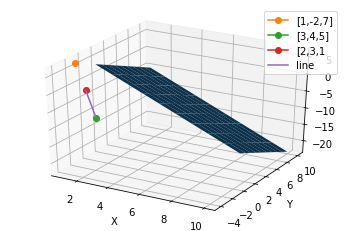
\includegraphics{Figure_3}
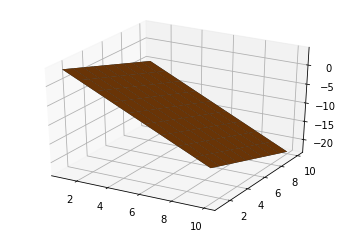
\includegraphics{Figure_4}






%\end{multicols}

\end{document}